\documentclass[t]{beamer}
\usetheme{_ghpcCInUFPE}

\usepackage[UKenglish]{babel}
\usepackage[long,nodayofweek,level]{datetime}
\usepackage[latin1]{inputenc}
\usepackage{times}
\usepackage[T1]{fontenc}
\usepackage{amsthm}
\usepackage{amsmath}
\usepackage{pgf}
\usepackage{hyperref}
\usepackage{verbatim}

\usepackage[color]{coqdoc}
\usepackage{cspsymb}
\usepackage{bussproofs}

\usepackage{multicol}

\title[A THEORY FOR CSP IN COQ]
{\large{A THEORY FOR COMMUNICATING \\ SEQUENTIAL PROCESSES IN COQ}}

\author[CARLOS FREITAS]
{
	Carlos Alberto da Silva Carvalho de Freitas\\
	(casc2@cin.ufpe.br)\\
	[7mm]{\small Supervisor: Gustavo Carvalho}
}

\institute[]
{
	Universidade Federal de Pernambuco\\
	Centro de Inform\'atica, 50740-560, Brazil\\
}

\date[24th November, 2020]

\pgfdeclareimage[height=1cm]{figures/cin-ufpe}{figures/cin-ufpe}
\logo{\pgfuseimage{figures/cin-ufpe}}

\AtBeginSection[]
{
	\begin{frame}<beamer>{Agenda}
		\tableofcontents[currentsection,currentsubsection]
	\end{frame}
}

% Defining symbol for the CSP_Coq language.
\newcommand{\CSPcoq}{CSP\textsubscript{\textit{Coq}}}

\begin{document}

\begin{frame}
	\titlepage
\end{frame}

%%%%%%%%%%%%%%%%%%%%%%%%%%%%%%%%%%%%%%%%%%%%%%%%%%%
\section*{Introduction}
%%%%%%%%%%%%%%%%%%%%%%%%%%%%%%%%%%%%%%%%%%%%%%%%%%%

\begin{frame}{Introduction}
	Concurrent systems
	\begin{itemize}
		\item Parallel execution of components
		\item Deadlock, nondeterminism and other issues
		\item Testing cannot guarantee properties such as determinism
	\end{itemize}
	\vskip 0.2in
	CSP: a theory for Communicating Sequential Processes
	\begin{itemize}
		\item Clear and accurate description of concurrent systems
		\item Designs can be proven correct with respect to desired properties
	\end{itemize}
\end{frame}

\begin{frame}{Introduction}
	Refinement (model) checkers
	\begin{itemize}
		\item Analysis and verification of systems via state exploration
		\item FDR: most popular refinement checker for CSP
		\item State explosion problem
	\end{itemize}
	\vskip 0.2in
	Verifying properties by proof development
\end{frame}

\begin{frame}{Objectives}
	Main: \emph{``provide an initial formalisation of the CSP language in Coq.''}
	\vskip 0.2in
	Specific objectives
	\begin{itemize}
		\item Define the syntax of a subset of CSP in Coq
		\item Support for the LTS representation based on the SOS
		\item Verify traces refinement via property-based random testing
	\end{itemize}
\end{frame}

\begin{frame}{Main contributions}
	\begin{itemize}
		\item Abstract and concrete syntax for a subset of CSP operators\\[2ex]
		\item Contextual rules for CSP specifications\\[2ex]
		\item Operational semantics via the SOS approach\\[2ex]
		\item Inductive and functional definitions of LTSs and traces\\[2ex]
		\item LTS visualisation using GraphViz\\[2ex]
		\item Automation for checking contextual rules and is-a-trace relation\\[2ex]
		\item Traces refinement verification using Quickchick
	\end{itemize}
\end{frame}

\begin{frame}<beamer>{Agenda}
	\tableofcontents
\end{frame}

%%%%%%%%%%%%%%%%%%%%%%%%%%%%%%%%%%%%%%%%%%%%%%%%%%%
\section{Background}
%%%%%%%%%%%%%%%%%%%%%%%%%%%%%%%%%%%%%%%%%%%%%%%%%%%

\subsection{CSP}

\begin{frame}{CSP: Communicating Sequential Processes}
	Example: the cloakroom attendant\\[2ex]
	\begin{itemize}
		\item \CSPM{}
		\ttfamily
		\scriptsize
		\begin{tabbing}
			channel coat\_on, coat\_off, store, retrieve, request\_coat, eat\\
			SYS\=TEM =\\
			\>	coat\_off -> store -> request\_coat -> retrieve -> coat\_on -> SKIP\\
			\>	{[| \{coat\_off, request\_coat, coat\_on\} |]}\\
			\>	coat\_off -> eat -> request\_coat -> coat\_on -> SKIP
		\end{tabbing}
		\normalfont
		\normalsize

		\vskip 0.1in
		\item LTS
		\begin{figure}
			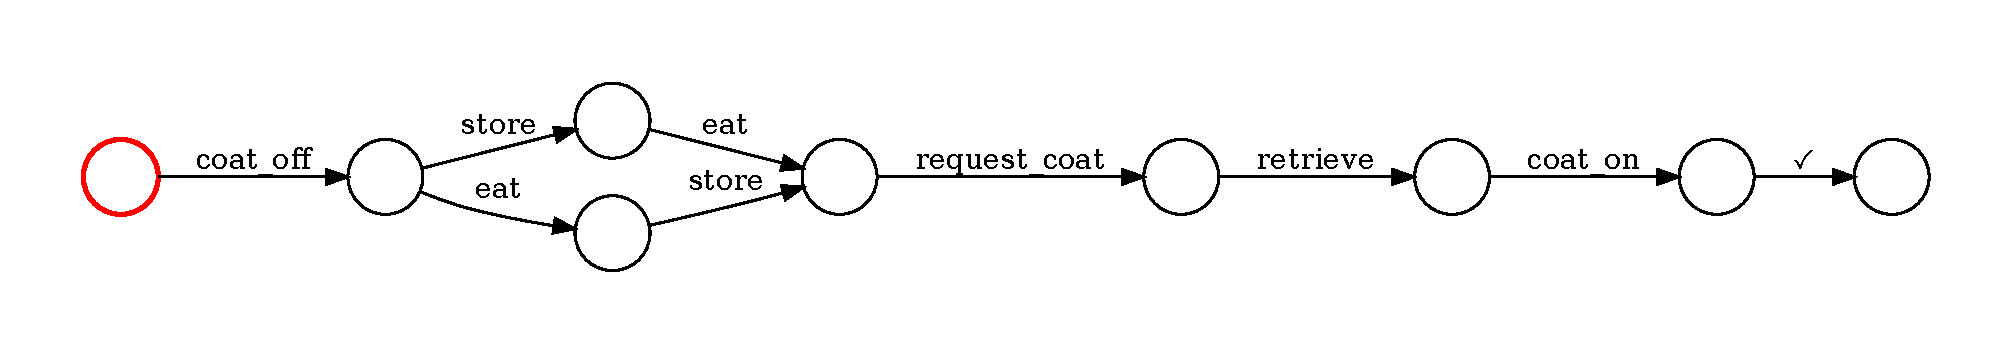
\includegraphics[scale=0.3]{figures/LTS.pdf}
		\end{figure}

		\item Traces
		\begin{itemize}
			\item $ \langle \mathit{coat\_off,\ store,\ eat} \rangle, $ \\
			$ \langle \mathit{coat\_off,\ eat,\ store,\ request\_coat} \rangle $\\
			$\ldots$
		\end{itemize}
	\end{itemize}
\end{frame}

\subsection{Coq}

\begin{frame}{Coq: a proof assistant}
	Functional and inductive definitions
	\vskip 0.1in
	\begin{columns}
		\scriptsize
		\column{0.5\textwidth}
		\begin{coqdoccode}
			\coqdocnoindent
			\coqdockw{Fixpoint} \coqdocvar{evenb} (\coqdocvar{n}:\coqdocvar{nat}) : \coqdocvar{bool} :=\coqdoceol
			\coqdocindent{1.00em}
			\coqdockw{match} \coqdocvar{n} \coqdockw{with}\coqdoceol
			\coqdocindent{2.00em}
			\ensuremath{|} \coqdocvar{O} \ensuremath{\Rightarrow} \coqdocvar{true}\coqdoceol
			\coqdocindent{2.00em}
			\ensuremath{|} \coqdocvar{S} \coqdocvar{O} \ensuremath{\Rightarrow} \coqdocvar{false}\coqdoceol
			\coqdocindent{2.00em}
			\ensuremath{|} \coqdocvar{S} (\coqdocvar{S} \coqdocvar{n'}) \ensuremath{\Rightarrow} \coqdocvar{evenb} \coqdocvar{n'}\coqdoceol
			\coqdocindent{1.00em}
			\coqdockw{end}.\coqdoceol
		\end{coqdoccode}
		\column{0.5\textwidth}
		\begin{coqdoccode}
			\coqdocnoindent
			\coqdockw{Inductive} \coqdocvar{ev} : \coqdocvar{nat} \ensuremath{\rightarrow} \coqdockw{Prop} :=\coqdoceol
			\coqdocindent{1.00em}
			\ensuremath{|} \coqdocvar{ev\_0} : \coqdocvar{ev} 0\coqdoceol
			\coqdocindent{1.00em}
			\ensuremath{|} \coqdocvar{ev\_SS} (\coqdocvar{n} : \coqdocvar{nat}) (\coqdocvar{H} : \coqdocvar{ev} \coqdocvar{n}) : \coqdocvar{ev} (\coqdocvar{S} (\coqdocvar{S} \coqdocvar{n})).\coqdoceol
		\end{coqdoccode}
	\end{columns}

	\vskip 0.2in
	Proof development and the tactics language Ltac
	\vskip 0.1in
	\begin{columns}[T]
		\scriptsize
		\column{0.5\textwidth}
		\begin{coqdoccode}
			\coqdocemptyline
			\coqdocnoindent
			\coqdockw{Lemma} \coqdocvar{negb\_involutive} : \coqdockw{\ensuremath{\forall}} (\coqdocvar{b} : \coqdocvar{bool}),\coqdoceol
			\coqdocindent{1.00em}
			\coqdocvar{negb} (\coqdocvar{negb} \coqdocvar{b}) = \coqdocvar{b}.\coqdoceol
			\coqdocnoindent
			\coqdockw{Proof}.\coqdoceol
			\coqdocindent{1.00em}
			\coqdoctac{destruct} \coqdocvar{b}.\coqdoceol
			\coqdocindent{1.00em}
			- \coqdoctac{simpl}. \coqdoctac{reflexivity}.\coqdoceol
			\coqdocindent{1.00em}
			- \coqdoctac{simpl}. \coqdoctac{reflexivity}.\coqdoceol
			\coqdocnoindent
			\coqdockw{Qed}.\coqdoceol
		\end{coqdoccode}
		\column{0.5\textwidth}
		\begin{coqdoccode}
			\coqdockw{Ltac} \coqdocvar{solve\_negb\_inv} \coqdocvar{b} :=\coqdoceol
			\coqdocindent{1.00em}
			\coqdoctac{destruct} \coqdocvar{b}; \coqdoctac{simpl}; \coqdoctac{reflexivity}.\coqdoceol
		\end{coqdoccode}
	\end{columns}
\end{frame}

\subsection{QuickChick}

\begin{frame}{QuickChick: a property-based testing tool}
	Example
	\vskip 0.1in
	\small
	\begin{coqdoccode}
		\coqdocnoindent
		\coqdockw{Fixpoint} \coqdocvar{remove} (\coqdocvar{x} : \coqdocvar{nat}) (\coqdocvar{l} : \coqdocvar{list} \coqdocvar{nat}) : \coqdocvar{list} \coqdocvar{nat} :=\coqdoceol
		\coqdocindent{1.00em}
		\coqdockw{match} \coqdocvar{l} \coqdockw{with}\coqdoceol
		\coqdocindent{2.00em}
		\ensuremath{|} []   \ensuremath{\Rightarrow} []\coqdoceol
		\coqdocindent{2.00em}
		\ensuremath{|} \coqdocvar{h}::\coqdocvar{t} \ensuremath{\Rightarrow} \coqdockw{if} \coqdocvar{h} =? \coqdocvar{x} \coqdockw{then} \coqdocvar{t} \coqdockw{else} \coqdocvar{h} :: \coqdocvar{remove} \coqdocvar{x} \coqdocvar{t}\coqdoceol
		\coqdocindent{1.00em}
		\coqdockw{end}.\coqdoceol
		\coqdocemptyline
		\coqdocnoindent
		\coqdockw{Conjecture} \coqdocvar{removeP} : \coqdockw{\ensuremath{\forall}} \coqdocvar{x} \coqdocvar{l},  \ensuremath{\lnot} (\coqdocvar{In} \coqdocvar{x} (\coqdocvar{remove} \coqdocvar{x} \coqdocvar{l})).\coqdoceol
		\coqdocemptyline
		\coqdocnoindent
		\coqdocvar{QuickChick} \coqdocvar{removeP}.\coqdoceol
	\end{coqdoccode}

	\vskip 0.2in
	\normalsize
	Output
	\vskip 0.1in
	\ttfamily
	\small
	0\\
	{[0, 0]}\\
	Failed! After 17 tests and 12 shrinks
\end{frame}

%%%%%%%%%%%%%%%%%%%%%%%%%%%%%%%%%%%%%%%%%%%%%%%%%%%
\section{A theory for CSP in Coq}
%%%%%%%%%%%%%%%%%%%%%%%%%%%%%%%%%%%%%%%%%%%%%%%%%%%

\subsection{Abstract and concrete syntax}

\begin{frame}{Abstract and concrete syntax}
	Event prefix
	\vskip 0.1in
	\begin{columns}
		\column{0.5\textwidth}
		\centering\small
		Abstract\\
		\texttt{ProcPrefix (Event ``e'') STOP}

		\column{0.5\textwidth}
		\centering\small
		Concrete\\
		\texttt{``e'' -{}-> STOP}
	\end{columns}

	\vskip 0.25in
	Example: process ``PRINTER''
	\begin{itemize}
		\item \CSPcoq{}\\
		\vskip 0.1in
		\begin{columns}
			\column{0.5\textwidth}
			\centering\small
			Abstract\\
			\ttfamily
			\begin{tabbing}
				P\=r\=o\=c\=\ ``PRINTER''\\
				\>	(ProcPrefix (Event ``accept'')\\
				\>\>	(ProcPrefix (Event ``print'')\\
				\>\>\>		STOP))
			\end{tabbing}
			\normalfont

			\column{0.5\textwidth}
			\centering\small
			Concrete\\
			\texttt{``PRINTER'' ::= ``accept'' -{}-> ``print'' -{}-> STOP}
		\end{columns}
		\vspace{1mm}
		\item \CSPM{}
		\vskip 0.05in
		\texttt{PRINTER = accept ->\\ $\ \ \ \ $ print -> STOP}
	\end{itemize}
\end{frame}

\begin{frame}{Abstract and concrete syntax}
	\begin{table}[htb]
		\scriptsize
		\begin{center}
			\begin{tabular}{ |l||c|c| }
				\hline
				\textbf{Constructor} & \textbf{\CSPM{}} & \textbf{\CSPcoq{}} \\
				\hline\hline
				Stop & STOP & STOP \\ [0.5ex]
				Skip & SKIP & SKIP \\ [0.5ex]
				Event prefix & e -> P & e -{}-> P \\  [0.5ex]
				External choice & P [] Q & P [] Q \\  [0.5ex]
				Internal choice & P |$ \sim $| Q & P |$ \sim $| Q \\ [0.5ex]
				Alphabetised parallel & P [A || B] Q & P [[A \textbackslash\textbackslash \ B]] Q \\ [0.5ex]
				Generalised parallel & P [| A |] Q & P [| A |] Q \\ [0.5ex]
				Interleave & P ||| Q & P ||| Q \\ [0.5ex]
				Sequential composition & P ; Q & P ;; Q \\ [0.5ex]
				Event hiding & P \textbackslash \ A & P \textbackslash \ A \\ [0.5ex]
				Process definition & P = Q & P ::= Q \\ [0.5ex]
				Process name & P & ProcRef ``P'' \\ [0.5ex]
				\hline
			\end{tabular}
		\end{center}
	\end{table}
\end{frame}

\begin{frame}{Abstract and concrete syntax}
	\begin{coqdoccode}
		\scriptsize
		\coqdocnoindent
		\coqdockw{Record} \coqdocvar{specification} : \coqdockw{Type} := \coqdocvar{Build\_Spec}\coqdoceol
		\coqdocnoindent
		\{\coqdoceol
		\coqdocindent{1.00em}
		\coqdocvar{ch\_list} : \coqdocvar{list} \coqdocvar{channel};\coqdoceol
		\coqdocindent{1.00em}
		\coqdocvar{proc\_list} : \coqdocvar{list} \coqdocvar{proc\_def};\coqdoceol
		\coqdocindent{1.00em}
		\coqdocvar{non\_empty\_proc\_ids} : \ensuremath{\lnot} \coqdocvar{In} \coqdocvar{EmptyString} (\coqdocvar{map} \coqdocvar{get\_proc\_id} \coqdocvar{proc\_list});\coqdoceol
		\coqdocindent{1.00em}
		\coqdocvar{non\_empty\_events} : \ensuremath{\lnot} \coqdocvar{In} \coqdocvar{EmptyString} (\coqdocvar{concat\_channels} \coqdocvar{ch\_list});\coqdoceol
		\coqdocindent{1.00em}
		\coqdocvar{no\_dup\_events\_proc\_ids} : \coqdocvar{NoDup} ((\coqdocvar{concat\_channels} \coqdocvar{ch\_list}) ++ (\coqdocvar{map} \coqdocvar{get\_proc\_id} \coqdocvar{proc\_list}));\coqdoceol
		\coqdocindent{1.00em}
		\coqdocvar{no\_missing\_proc\_defs} : \coqdocvar{incl} (\coqdocvar{get\_proc\_refs} \coqdocvar{proc\_list}) (\coqdocvar{map} \coqdocvar{get\_proc\_id} \coqdocvar{proc\_list});\coqdoceol
		\coqdocindent{1.00em}
		\coqdocvar{no\_missing\_events} : \coqdocvar{incl} (\coqdocvar{get\_events} \coqdocvar{proc\_list}) (\coqdocvar{concat\_channels} \coqdocvar{ch\_list})\coqdoceol
		\coqdocnoindent
		\}.\coqdoceol
		\coqdocemptyline
		\coqdocnoindent
		\coqdockw{Ltac} \coqdocvar{solve\_spec\_ctx\_rules} \coqdocvar{spec\_cons} := \coqdoctac{apply} \coqdocvar{spec\_cons};\coqdoceol
		\coqdocindent{1.00em}
		\coqdoctac{repeat} (\coqdoceol
		\coqdocindent{2.00em}
		\coqdockw{match} \coqdockw{goal} \coqdockw{with}\coqdoceol
		\coqdocindent{2.00em}
		\ensuremath{|} \ensuremath{\vdash} \ensuremath{\lnot} \coqdocvar{In} \coqdocvar{\_} \coqdocvar{\_} \ensuremath{\Rightarrow} \coqdocvar{solve\_not\_in}\coqdoceol
		\coqdocindent{2.00em}
		\ensuremath{|} \ensuremath{\vdash} \coqdocvar{NoDup} \coqdocvar{\_} \ensuremath{\Rightarrow} \coqdocvar{solve\_nodup}\coqdoceol
		\coqdocindent{2.00em}
		\ensuremath{|} \ensuremath{\vdash} \coqdocvar{incl} \coqdocvar{\_} \coqdocvar{\_} \ensuremath{\Rightarrow} \coqdocvar{solve\_incl}\coqdoceol
		\coqdocindent{2.00em}
		\coqdockw{end}\coqdoceol
		\coqdocindent{1.00em}
		); \coqdoctac{fail} "One or more contextual rules were not fulfilled".\coqdoceol
	\end{coqdoccode}
\end{frame}

\subsection{Structured Operational Semantics}

\begin{frame}{Structured Operational Semantics}
	Inference rule
	\vskip 0.1in
	\begin{columns}
		\column{0.5\textwidth}
		\centering\small
		Event prefix\\
		\begin{prooftree}
			\AxiomC{}
			\UnaryInfC{$ (a \then P) \trans(2)[a] P $}
		\end{prooftree}

		\column{0.5\textwidth}
		\centering\small
		External choice\\
		\begin{prooftree}
			\AxiomC{$ P \trans(2)[a] P' $}
			\RightLabel{\quad ($ a \neq \tau $)}
			\UnaryInfC{$ P \extchoice Q \trans(2)[a] P' $}
		\end{prooftree}
	\end{columns}
	\vskip 0.2in
	Inductive definition: \coqdocvar{sosR}
	\vskip 0.05in
	\small
	\begin{coqdoccode}
		\coqdocnoindent
		\coqdockw{Inductive} \coqdocvar{sosR} : \coqdocvar{specification} \ensuremath{\rightarrow}\coqdoceol
		\coqdocindent{1.00em}\coqdocvar{proc\_body} \ensuremath{\rightarrow} \coqdocvar{event\_tau\_tick} \ensuremath{\rightarrow} \coqdocvar{proc\_body} \ensuremath{\rightarrow} \coqdockw{Prop} :=\coqdoceol
		\coqdocindent{1.00em}
		\ensuremath{|} \coqdocvar{prefix\_rule} (\coqdocvar{S} : \coqdocvar{specification}) (\coqdocvar{P} : \coqdocvar{proc\_body}) (\coqdocvar{a} : \coqdocvar{event}) :\coqdoceol
		\coqdocindent{1.50em}
		\coqdocvar{S} \# (\coqdocvar{a} \texttt{-{}-}> \coqdocvar{P}) // \coqdocvar{Event} \coqdocvar{a} ==> \coqdocvar{P}\coqdoceol
		\coqdocindent{1.00em}
		\ensuremath{|} \coqdocvar{ext\_choice\_left\_rule} (\coqdocvar{S} : \coqdocvar{specification}) (\coqdocvar{P} \coqdocvar{Q} : \coqdocvar{proc\_body}) :\coqdoceol
		\coqdocindent{1.50em}
		\coqdockw{\ensuremath{\forall}} (\coqdocvar{P'} : \coqdocvar{proc\_body}) (\coqdocvar{a} : \coqdocvar{event\_tau\_tick}),\coqdoceol
		\coqdocindent{3.00em}
		\ensuremath{\lnot} \coqdocvar{eq} \coqdocvar{a} \coqdocvar{Tau} \ensuremath{\rightarrow}\coqdoceol
		\coqdocindent{3.00em}
		(\coqdocvar{S} \# \coqdocvar{P} // \coqdocvar{a} ==> \coqdocvar{P'}) \ensuremath{\rightarrow}\coqdoceol
		\coqdocindent{3.00em}
		(\coqdocvar{S} \# \coqdocvar{P} [] \coqdocvar{Q} // \coqdocvar{a} ==> \coqdocvar{P'})
	\end{coqdoccode}
\end{frame}

\subsection{Labelled Transition Systems}

\begin{frame}{Labelled Transition Systems}
	Propositional function \coqdocvar{ltsR}
	\vskip 0.1in
	\begin{coqdoccode}
		\coqdocnoindent
		\coqdockw{Definition} \coqdocvar{ltsR} (\coqdocvar{S} : \coqdocvar{specification}) (\coqdocvar{name} : \coqdocvar{string}) (\coqdocvar{T} : \coqdoctac{set} \coqdocvar{transition}) : \coqdockw{Prop} :=\coqdoceol
		\coqdocindent{1.00em}
		\coqdockw{match} \coqdocvar{get\_proc\_body} \coqdocvar{S} \coqdocvar{name} \coqdockw{with}\coqdoceol
		\coqdocindent{1.00em}
		\ensuremath{|} \coqdocvar{Some} \coqdocvar{body} \ensuremath{\Rightarrow} \coqdocvar{NoDup} \coqdocvar{T} \ensuremath{\land} \coqdocvar{ltsR'} \coqdocvar{S} \coqdocvar{T} [\coqdocvar{body}] \coqdocvar{nil}\coqdoceol
		\coqdocindent{1.00em}
		\ensuremath{|} \coqdocvar{None} \ensuremath{\Rightarrow} \coqdocvar{False}\coqdoceol
		\coqdocindent{1.00em}
		\coqdockw{end}.\coqdoceol
	\end{coqdoccode}
\end{frame}

\begin{frame}{Labelled Transition Systems}
	Inductive definition: \coqdocvar{ltsR'}
	\vskip 0.1in
	\begin{coqdoccode}
		\coqdocnoindent
		\coqdockw{Inductive} \coqdocvar{ltsR'} : \coqdocvar{specification} \ensuremath{\rightarrow} \coqdoctac{set} \coqdocvar{transition} \ensuremath{\rightarrow} \coqdoctac{set} \coqdocvar{proc\_body} \ensuremath{\rightarrow} \coqdoctac{set} \coqdocvar{proc\_body} \ensuremath{\rightarrow} \coqdockw{Prop}.\coqdoceol
	\end{coqdoccode}
	\vskip 0.2in
	\begin{itemize}
		\item \coqdocvar{lts\_empty\_rule}: no states remain to be visited; the corresponding LTS is empty
		\item \coqdocvar{lts\_inductive\_rule}: for all process states, it is valid operation according to the SOS, if, and only if, the corresponding 3-tuple belongs to the set of transitions
	\end{itemize}
\end{frame}

\begin{frame}{Labelled Transition Systems}
	Functional definitions: \coqdocvar{compute\_ltsR} and \coqdocvar{generate\_dot}
	\vskip 0.1in
	\begin{coqdoccode}
		\scriptsize
		\coqdocnoindent
		\coqdockw{Definition} \coqdocvar{compute\_ltsR}\coqdoceol
		\coqdocindent{1.00em}
		(\coqdocvar{S} : \coqdocvar{specification}) (\coqdocvar{name} : \coqdocvar{string}) (\coqdocvar{limit} : \coqdocvar{nat}) : \coqdocvar{option} (\coqdoctac{set} \coqdocvar{transition}).\coqdoceol
		\coqdocemptyline
		\coqdocnoindent
		\coqdockw{Definition} \coqdocvar{generate\_dot} (\coqdocvar{lts} : \coqdocvar{option} (\coqdoctac{set} \coqdocvar{transition})) : \coqdocvar{string}.\coqdoceol
	\end{coqdoccode}
	\vskip 0.2in
	Example: process ``MACHINE''
	\vskip 0.1in
	\begin{coqdoccode}
		\scriptsize
		\coqdocnoindent
		\coqdockw{Definition} \coqdocvar{PARKING\_PERMIT\_MCH} : \coqdocvar{specification}.\coqdoceol
		\coqdocnoindent
		\coqdockw{Proof}.\coqdoceol
		\coqdocindent{1.00em}
		\coqdocvar{solve\_spec\_ctx\_rules} (\coqdoceol
		\coqdocindent{2.00em}
		\coqdocvar{Build\_Spec}\coqdoceol
		\coqdocindent{2.00em}
		[ \coqdocvar{Channel} \{\{``cash'', ``ticket'', ``change''\}\} ]\coqdoceol
		\coqdocindent{2.00em}
		[ ``TICKET'' ::= ``cash'' -{}-> ``ticket'' -{}-> \coqdocvar{ProcRef} ``TICKET''\coqdoceol
		\coqdocindent{2.00em}
		; ``CHANGE'' ::= ``cash'' -{}-> ``change'' -{}-> \coqdocvar{ProcRef} ``CHANGE''\coqdoceol
		\coqdocindent{2.00em}
		; ``MACHINE'' ::= \coqdocvar{ProcRef} ``TICKET''\coqdoceol
		\coqdocindent{10.50em}[[ \{\{``cash'', ``ticket''\}\} \symbol{92}\symbol{92} \{\{``cash'', ``change''\}\} ]]\coqdoceol
		\coqdocindent{10.50em}\coqdocvar{ProcRef} ``CHANGE'' ]\coqdoceol
		\coqdocindent{1.00em}
		).\coqdoceol
		\coqdocnoindent
		\coqdockw{Defined}.\coqdoceol
	\end{coqdoccode}
\end{frame}

\begin{frame}{Labelled Transition Systems}
	Graph visualisation (GraphViz)
	\begin{figure}
		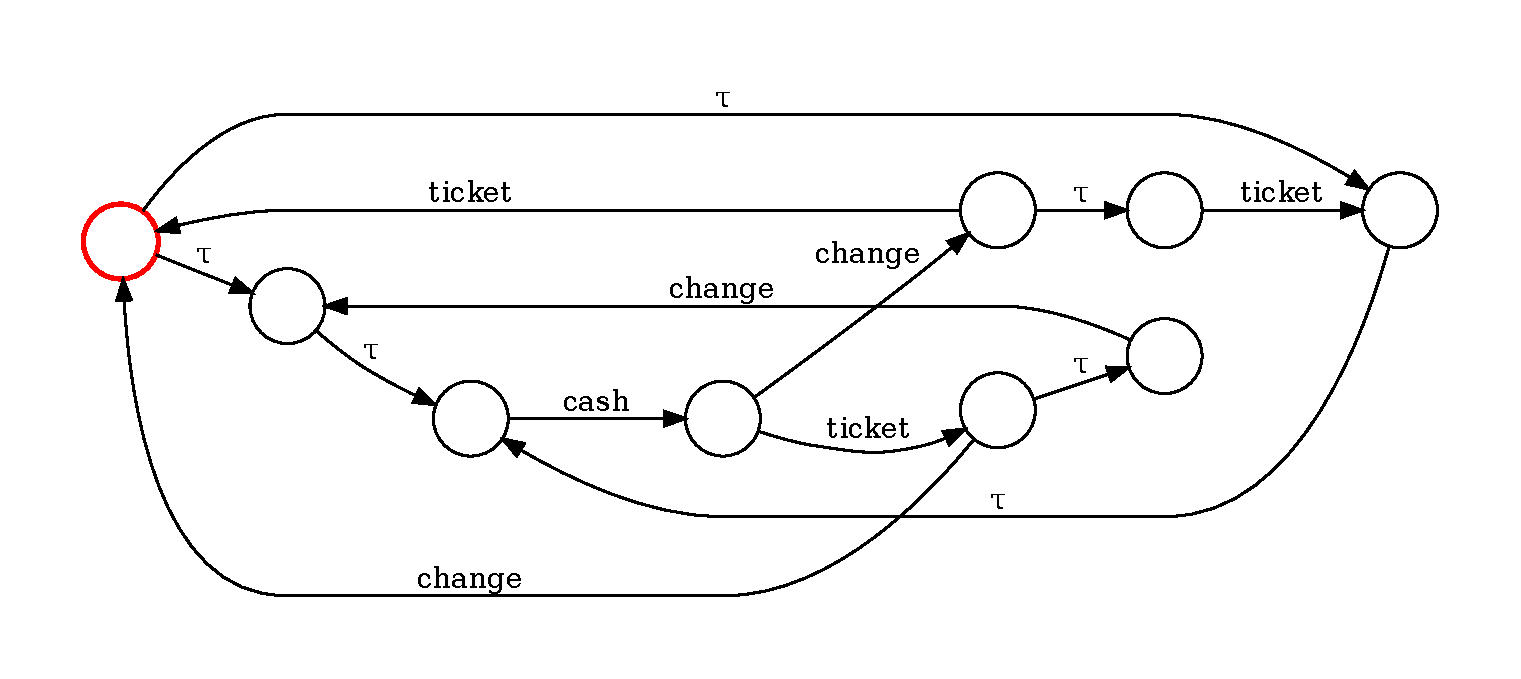
\includegraphics[scale=0.4]{figures/MACHINE_LTS.pdf}
	\end{figure}
\end{frame}

\subsection{Traces refinement}

\begin{frame}{Is-a-trace relation}
	Inductive definition: \coqdocvar{traceR'}
	\vskip 0.1in
	\begin{coqdoccode}
		\small
		\coqdocnoindent
		\coqdockw{Inductive} \coqdocvar{traceR'} : \coqdocvar{specification} \ensuremath{\rightarrow} \coqdocvar{proc\_body} \ensuremath{\rightarrow} \coqdocvar{trace} \ensuremath{\rightarrow} \coqdockw{Prop}.\coqdoceol
	\end{coqdoccode}
	\begin{itemize}
		\item \coqdocvar{empty\_trace\_rule}
		\item \coqdocvar{event\_trace\_rule}
		\item \coqdocvar{tau\_trace\_rule}
	\end{itemize}
	\vskip 0.2in
	Proof automation for the is-a-trace relation: \coqdocvar{solve\_trace}
	\vskip 0.1in
	\begin{coqdoccode}
		\small
		\coqdocnoindent
		\coqdockw{Example} \coqdocvar{MACHINE\_TRACE} :\coqdoceol
		\coqdocindent{1.00em}
		\coqdocvar{traceR} \coqdocvar{PARKING\_PERMIT\_MCH} ``MACHINE'' [``cash'' ; ``ticket'' ; ``change''].\coqdoceol
		\coqdocnoindent
		\coqdockw{Proof}. \coqdocvar{solve\_trace}. \coqdockw{Qed}.\coqdoceol
	\end{coqdoccode}
\end{frame}

\begin{frame}{Traces refinement}
	Traces refinement formalisation
	\vskip 0.1in
	\begin{coqdoccode}
		\small
		\coqdocnoindent
		\coqdockw{Definition} \coqdocvar{trace\_refinement}\coqdoceol
		\coqdocindent{0.50em}(\coqdocvar{S} : \coqdocvar{specification}) (\coqdocvar{Spec} \coqdocvar{Imp} : \coqdocvar{string}) : \coqdockw{Prop} :=\coqdoceol
		\coqdocindent{1.00em}
		\coqdockw{\ensuremath{\forall}} (\coqdocvar{t} : \coqdocvar{trace}), \coqdocvar{traceR} \coqdocvar{S} \coqdocvar{Imp} \coqdocvar{t} \ensuremath{\rightarrow} \coqdocvar{traceR} \coqdocvar{S} \coqdocvar{Spec} \coqdocvar{t}.\coqdoceol
		\coqdocemptyline
		\coqdocnoindent
		\coqdockw{Notation} ``S `\#' P `[T=' Q'' := (\coqdocvar{trace\_refinement} \coqdocvar{S} \coqdocvar{P} \coqdocvar{Q})\coqdoceol
		\coqdocindent{1.00em}
		(\coqdoctac{at} \coqdockw{level} 150, \coqdoctac{left} \coqdockw{associativity}).\coqdoceol
	\end{coqdoccode}
\end{frame}

\begin{frame}{Traces refinement}
	Traces generator: \coqdocvar{gen\_valid\_trace'}
	\vskip 0.1in
	\begin{columns}[T]
		\column{0.55\textwidth}
		\begin{coqdoccode}
			\scriptsize
			\coqdocnoindent
			\coqdockw{Fixpoint} \coqdocvar{gen\_valid\_trace'}\coqdoceol
			\coqdocindent{1.00em}
			(\coqdocvar{S} : \coqdocvar{specification}) (\coqdocvar{P} : \coqdocvar{proc\_body}) (\coqdocvar{size} : \coqdocvar{nat})\coqdoceol
			\coqdocindent{1.00em}
			: \coqdocvar{G} (\coqdocvar{option} \coqdocvar{semantics\_trace.trace}) :=\coqdoceol
			\coqdocindent{1.00em}
			\coqdockw{match} \coqdocvar{size} \coqdockw{with}\coqdoceol
			\coqdocindent{1.00em}
			\ensuremath{|} \coqdocvar{O} \ensuremath{\Rightarrow} \coqdocvar{ret} \coqdocvar{nil}\coqdoceol
			\coqdocindent{1.00em}
			\ensuremath{|} \coqdocvar{S} \coqdocvar{size'} \ensuremath{\Rightarrow}\coqdoceol
			\coqdocindent{2.00em}
			\coqdocvar{freq\_} (\coqdocvar{ret} \coqdocvar{nil}) [\coqdoceol
			\coqdocindent{3.00em}
			(1, \coqdocvar{ret} \coqdocvar{nil}) ;\coqdoceol
			\coqdocindent{3.00em}
			(\coqdocvar{size},\coqdoceol
			\coqdocindent{4.00em}
			\coqdocvar{bind} (\coqdocvar{gen\_valid\_trans} \coqdocvar{S} \coqdocvar{P}) (\coqdoceol
			\coqdocindent{5.00em}
			\coqdockw{fun} \coqdocvar{t} \ensuremath{\Rightarrow} (\coqdoceol
			\coqdocindent{6.00em}
			\coqdockw{match} \coqdocvar{t} \coqdockw{with}\coqdoceol
			\coqdocindent{6.00em}
			\ensuremath{|} \coqdocvar{nil} \ensuremath{\Rightarrow} \coqdocvar{ret} \coqdocvar{nil}\coqdoceol
			\coqdocindent{6.00em}
			\ensuremath{|} (\coqdocvar{Event} \coqdocvar{e}, \coqdocvar{Q}) :: \coqdocvar{\_} \ensuremath{\Rightarrow}\coqdoceol
			\coqdocindent{7.00em}
			\coqdocvar{bind} (\coqdocvar{gen\_valid\_trace'} \coqdocvar{S} \coqdocvar{Q} \coqdocvar{size'}) (\coqdoceol
			\coqdocindent{8.00em}
			\coqdockw{fun} \coqdocvar{ts} \ensuremath{\Rightarrow} \coqdocvar{ret} (\coqdocvar{Event} \coqdocvar{e} :: \coqdocvar{ts})\coqdoceol
			\coqdocindent{7.00em}
			)\coqdoceol
		\end{coqdoccode}

		\column{0.45\textwidth}
		\begin{coqdoccode}
			\scriptsize
			\coqdocindent{1.00em}
			\ensuremath{|} (\coqdocvar{Tick}, \coqdocvar{Q}) :: \coqdocvar{\_} \ensuremath{\Rightarrow}\coqdoceol
			\coqdocindent{2.00em}
			\coqdocvar{bind} (\coqdocvar{gen\_valid\_trace'} \coqdocvar{S} \coqdocvar{Q} \coqdocvar{size'}) (\coqdoceol
			\coqdocindent{3.00em}
			\coqdockw{fun} \coqdocvar{ts} \ensuremath{\Rightarrow} \coqdocvar{ret} (\coqdocvar{Tick} :: \coqdocvar{ts})\coqdoceol
			\coqdocindent{2.00em}
			)\coqdoceol
			\coqdocindent{1.00em}
			\ensuremath{|} (\coqdocvar{Tau}, \coqdocvar{Q}) :: \coqdocvar{\_} \ensuremath{\Rightarrow}\coqdoceol
			\coqdocindent{2.00em}
			\coqdocvar{bind} (\coqdocvar{gen\_valid\_trace'} \coqdocvar{S} \coqdocvar{Q} \coqdocvar{size'}) (\coqdoceol
			\coqdocindent{3.00em}
			\coqdockw{fun} \coqdocvar{ts} \ensuremath{\Rightarrow} \coqdocvar{ret} \coqdocvar{ts}\coqdoceol
			\coqdocindent{2.00em}
			)\coqdoceol
			\coqdocindent{1.00em}
			\coqdockw{end}\coqdoceol
			) ) ) ]	\coqdockw{end}.\coqdoceol
		\end{coqdoccode}
	\end{columns}
\end{frame}

\begin{frame}{Traces refinement}
	Demonstrating the random generator of valid traces
	\vskip 0.1in
	\small
	\begin{coqdoccode}
		\coqdocnoindent
		\coqdocvar{Sample} (\coqdocvar{gen\_valid\_trace} \coqdocvar{PARKING\_PERMIT\_MCH} ``MACHINE'' 10).\coqdoceol
	\end{coqdoccode}
	\vskip 0.2in
	Output:
	\vskip 0.1in
	\ttfamily
	{[Some []; Some [``cash''; ``change''; ``ticket''; ``cash''; ``change'']};
	{Some [``cash'']; Some [``cash''; ``ticket''; ``change''; ``cash'']; Some []};
	{Some [``cash''; ``change''; ``ticket''; ``cash'']; Some [``cash''; ``change''; ``ticket'']; $\dots$]}
\end{frame}

\begin{frame}{Traces refinement}
	Executable property: \coqdocvar{traceP}
	\vskip 0.1in
	\begin{coqdoccode}
		\small
		\coqdocnoindent
		\coqdockw{Definition} \coqdocvar{traceP}\coqdoceol
		\coqdocindent{1.00em}
		(\coqdocvar{S} : \coqdocvar{specification})\coqdoceol
		\coqdocindent{1.00em}
		(\coqdocvar{proc\_id} : \coqdocvar{string})\coqdoceol
		\coqdocindent{1.00em}
		(\coqdocvar{fuel} : \coqdocvar{nat})\coqdoceol
		\coqdocindent{1.00em}
		(\coqdocvar{t} : \coqdocvar{option} \coqdocvar{semantics\_trace.trace}) : \coqdocvar{bool}.\coqdoceol
	\end{coqdoccode}
	\vskip 0.2in
	Refinement checker: \coqdocvar{trace\_refinement\_checker}
	\vskip 0.1in
	\begin{coqdoccode}
		\small
		\coqdocnoindent
		\coqdockw{Definition} \coqdocvar{trace\_refinement\_checker}\coqdoceol
		\coqdocindent{1.00em}
		(\coqdocvar{S} : \coqdocvar{specification})\coqdoceol
		\coqdocindent{1.00em}
		(\coqdocvar{Imp} \coqdocvar{Spec} : \coqdocvar{string})\coqdoceol
		\coqdocindent{1.00em}
		(\coqdocvar{trace\_max\_size} : \coqdocvar{nat})\coqdoceol
		\coqdocindent{1.00em}
		(\coqdocvar{fuel} : \coqdocvar{nat}) : \coqdocvar{Checker} :=\coqdoceol
		\coqdocindent{2.00em}
		\coqdocvar{forAll} (\coqdocvar{gen\_valid\_trace} \coqdocvar{S} \coqdocvar{Imp} \coqdocvar{trace\_max\_size})\coqdoceol
		\coqdocindent{3.00em}(\coqdocvar{traceP} \coqdocvar{S} \coqdocvar{Spec} \coqdocvar{fuel}).\coqdoceol
	\end{coqdoccode}
\end{frame}

\begin{frame}{Traces refinement}
	Searching for counterexamples with QuickChick
	\vskip 0.1in
	\small
	\begin{coqdoccode}
		\coqdocnoindent
		\coqdockw{Definition} \coqdocvar{EXAMPLE} : \coqdocvar{specification}.\coqdoceol
		\coqdocnoindent
		\coqdockw{Proof}.\coqdoceol
		\coqdocindent{1.00em}
		\coqdocvar{solve\_spec\_ctx\_rules} (\coqdoceol
		\coqdocindent{2.00em}
		\coqdocvar{Build\_Spec}\coqdoceol
		\coqdocindent{3.00em}
		[ \coqdocvar{Channel} \{\{``a'', ``b'', ``c''\}\} ]\coqdoceol
		\coqdocindent{3.00em}
		[ ``P'' ::= ``a'' -{}-> ``b'' -{}-> \coqdocvar{ProcRef} ``P'' ;\coqdoceol
		\coqdocindent{4.00em}
		``Q'' ::= (``a'' -{}-> ``b'' -{}-> \coqdocvar{ProcRef} ``Q'') [] (``c'' -{}-> \coqdocvar{STOP}) ]\coqdoceol
		\coqdocindent{1.00em}
		).\coqdoceol
		\coqdocnoindent
		\coqdockw{Defined}.\coqdoceol
		\coqdocemptyline
		\coqdocnoindent
		\coqdocvar{QuickChick} (\coqdocvar{trace\_refinement\_checker} \coqdocvar{EXAMPLE} ``Q'' ``P'' 5 1000).\coqdoceol
	\end{coqdoccode}
	\vskip 0.2in
	Output:
	\vskip 0.1in
	\ttfamily
	Some {[``c'']}\\
	*** Failed after 3 tests\\
	and 0 shrinks. (0 discards)
\end{frame}

%%%%%%%%%%%%%%%%%%%%%%%%%%%%%%%%%%%%%%%%%%%%%%%%%%%
\section{Conclusion}
%%%%%%%%%%%%%%%%%%%%%%%%%%%%%%%%%%%%%%%%%%%%%%%%%%%

\begin{frame}{Conclusion}
	$\CSPcoq{}$: an initial formalisation of the CSP language in Coq\\[1ex]
	\begin{itemize}
		\item Inductive and functional definitions of LTSs and traces\\[2ex]
		\item Third-party visualisation support for LTS representation\\[2ex]
		\item Automation for checking contextual rules and is-a-trace relation\\[2ex]
		\item Random testing for refinement relations using QuickChick
	\end{itemize}
\end{frame}

\subsection{Related work}

\begin{frame}{Related work}
	CSP-Prover
	\begin{itemize}
		\item Interactive theorem prover based on Isabelle
		\item Stable-failures model as the underlying denotational semantics
		\item Semi-automated proof tactics for refinement verification
	\end{itemize}
	\vskip 0.15in
	Isabelle/UTP
	\begin{itemize}
		\item Implementation of the \emph{Unifying Theories of Programming}
		\item Support for construction of denotational semantic meta-models
		\item Useful to construct program verification tools
	\end{itemize}
	\vskip 0.15in
	Distinguishable features of \CSPcoq{}
	\begin{itemize}
		\item Graphical representation of LTSs
		\item Property-based testing for\\checking traces refinement relations
	\end{itemize}
\end{frame}

\subsection{Future work}

\begin{frame}{Future work}
	\begin{itemize}
		\item Extend the \CSPcoq{} dialect to include other CSP operators\\[2ex]
		\item Check for invalid recursions (hiding and parallelism operations)\\[2ex]
		\item Define a tactic to automate proofs involving the relation \coqdocvar{ltsR}\\[2ex]
		\item Prove correctness of definition \coqdocvar{compute\_ltsR}\\[2ex]
		\item Prove correctness of generator \coqdocvar{gen\_valid\_trace}\\[2ex]
		\item Define traces refinement in terms of bi-simulation
	\end{itemize}
\end{frame}

\begin{frame}
	\titlepage
\end{frame}

\end{document}